\documentclass{article}
\usepackage{geometry}
\geometry{
        a4paper,
        total={170mm,257mm},
        left=20mm,
        top=20mm
}

\usepackage{graphicx}
\usepackage{subfig}
% \usepackage{subcaption}
\usepackage{caption}
% \usepackage{amsmath}

% \usepackage{longtable}


\newcommand{\imWidth}{5.5cm}




\title{Data Mining CW1}

\author{Merlin Lindsay\\
        \small  K20090065 
}
\date{}


\setlength{\arrayrulewidth}{0.2mm}
\setlength{\tabcolsep}{18pt}


\begin{document}
\maketitle

\section*{Introduction}

This report outlines the classification and cluster analysis undertaken as part of KCL Data Mining CW1. The report is is made up of
two sections. In Section 1, using the Adult dataset from Scikit-Learn, the handling of missing data values are explored in classifcation tasks. In Section 2,
using the Wholesale \& Customers dataset, also from Scikit-Learn, clustering is used to group similar instances from the data.


\section{Classification}

This section contains the use of the Adult dataset,comprised of information on adults over multiple attributes such as age, 
sex, occupation, and their corresponding income.



\subsection{Metadata}
The information extracted from this dataset, in relation to missing values, are shown in Table \ref{table:metAdult}.
\vspace{2mm}

\begin{table}
        \centering
\begin{tabular}{ |c|c|}
        \hline
        Metric & Value\\
        \hline
        Number of instances & 48842\\
        Number of missing values & 6465\\
        Fraction of missing values & 0.010\\
        Instances with missing values & 3620\\
        Fraction of instances missing values & 0.074\\
        \hline
       \end{tabular}
\caption{Metadata of Adult Dataset}
        \label{table:metAdult}
\end{table}

% \vspace{2mm}

Given roughly 7\% of the instances in the dataset are missing values, this presented a suitable opportunity to assess the impact 
that missing elements can have on data manipulation. The accompanying code must account for unexpected missing values
where necessary and convert them to usable data types, as will be shown in the following sections.


\subsection{Nominal Conversion}

To train the classifiers used in the report, the missing data-points must be converted to usable data-types, in the form of discrete values. 
To obtain the unique discrete values for each attribute, the data must be converted to categorical labels. The NaN value that represents the missing 
data-points in the dataset is of type floating-point. 
It is not possible to convert floating-point types to labels using the Scikit-Learn LabelEncoder, so the NaN values must be replaced with a string (or int type).
 In this case a placeholder string `missing' was used.
\vspace{2mm}

Using the label encoder, each of the values contained in the dataset were converted to a discrete numerical integer value. Each integer 
represents an attribute value for its respective column. It is important to note these integers represent only values containted within the 
dataset, and not other possible values that could occur despite not being present in the dataset. Numerical attributes
within the dataset would also be converted to discrete values, so this method should be avoided with continuous data types to prevent 
encoding problems when adding new data. This was not a problem for this report, as there were no continuous variables in this dataset.

\vspace{2mm}


The discrete values are shown in Table \ref{table:discVals}.
\begin{table}
        \centering
\begin{tabular}{ |c|c|}
        \hline
        Attribute & Discrete Value\\
        \hline
        
        age & 0 1 2 3 4\\
        workclass & 0 1 2 3 4 5 6 7 8\\
        education &  0 1 2 3 4 5 6 7 8 9 10 11 12 13 14 15\\
        education-num &  0  1  2  3  4  5  6  7  8  9 10 11 12 13 14 15\\
        marital-status & 0 1 2 3 4 5 6\\
        occupation & 0  1  2  3  4  5  6  7  8  9 10 11 12 13 14\\
        relationship & 0 1 2 3 4 5\\
        race & 0 1 2 3 4\\
        sex & 0 1\\
        capitalgain & 0 1 2 3 4\\
        capitalloss & 0 1 2 3 4\\
        hoursperweek & 0 1 2 3 4\\
        native-country & \shortstack{0 1 2 3 4 5 6 7 8 9 10 11 12 13 14 15 16 17 18 19 20 \\21 22 23 24 25 26 27 28 29 30 31 32 33 34 35 36 37 38 39 40 41}\\
        class & 0 1\\
        \hline
       \end{tabular}
\caption{Discrete Values of Attributes}
        \label{table:discVals}
\end{table}

\subsection{Classification Without Missing Values}

Ignoring any instance with missing values, that is to say any row containing NaN or `missing' values, a decision-tree classifier was trained
and its error rate computed. To do this, the NaN values were dropped, and the dataset encoded into discrete values. 
To train a classifier it is necessary to split the data into training and test sets. This is so the classifier's 
performance can be measured on data it has not yet seen, as it will be biased to perform well on data it was trained on, so a separate 
test set from a train set is used for performance evaluation. 
The encoded dataset had 10-fold cross validation performed on it, which provided an average error rate across the entire dataset. This involves
splitting the dataset in 10 different ways, and training and testing over each split. The average error rate can then be computed

\noindent The formula for calculating the error rate, as shwon in Table \ref{table:origErr} was as follows:

        
        \[Error Rate = 1 - \frac{1}{m} \sum_{i = 1}^{m} score_{i}\]
        



\begin{table}
        \centering
\begin{tabular}{ |c|c|}
        \hline
        Dataset trained on & Error Rate\\
        \hline
        D (dropped missing) & 0.173\\
        \hline
       \end{tabular}
\caption{Discrete Values of Attributes}
        \label{table:origErr}
\end{table}




\subsection{Handling Missing Values}

Given the abundance of missing values in the dataset, there are multiple approaches to handling the training of the classifier. In this case
two datasets were created from a subset of the original dataset. To create the subset, $D^{\prime}$, first every instance containing at leaset one missing value was extracted from the dataset. Next, an equal number of instances containing no
missing values were extracted.

\vspace{2mm}
The first dataset from the subset, $D^{\prime}_{1}$, was created by simply replacing every NaN value in $D^{\prime}$ with a string; `missing'.
The second dataset from the subset, $D^{\prime}_{2}$, was created by replacing the NaN values in $D^{\prime}$ with modal value for the respective attribute.

\vspace{2mm}
Two decision trees were trained on one of these datasets each. Then, using $D$ (the original dataset) for testing, which contained no missing values, 
the error rate was calculated on this unseen data. To facilitate a direct comparison between these two classifiers and the classifier from Section 1.3,
the classifiers were tested on the entire dataset $D$.

\vspace{2mm}

The error rates for the classifiers are shown in Table \ref{table:errs}.

\begin{table}
{
        \centering
        \begin{tabular}{|c|c|}
        \hline
        Dataset trained on & Error Rate on D\\
        \hline
        $D^{\prime}_{1}$ & 0.171\\ 
        $D^{\prime}_{2}$ & 0.181\\
        \hline
       \end{tabular}
\caption{Error Rates of Missing-Value Trees}
        \label{table:errs}
}
\end{table}


\vspace{4mm}
Once again these error values will change with each run of the code, though it should be noted the classifier trained on $D^{\prime}_{1}$ consistently 
scored better than the one trained on $D^{\prime}_{2}$. $D^{\prime}_{1}$ had similar performance to the classifier trained on dataset $D$ (the classifier from 1.3), with instances missing values 
removed. This gives rise to several points to note.\\

It could be that the missing-value-handling method of replacing missing values with modal values has a negative effect on the performance of classifiers
on unseen data, i.e., manipulating the data in this way may hinder the accuracy of models.

Given the classifiers were trained on data where 50\% of instances had at least one missing value, it is possible there was bias in the 
training, as only 7\% of the testing examples contained missing data.\\

As an alternative means of evaluating the performace of the classifier models, k-fold cross validation could have been used on these new datasets. This would assess the 
average score of the models over the respective datasets, as opposed to the full dataset $D$ with examples unrepresentative of those they were trained on.



\section{Clustering} 

This section uses data from a wholesale distributer, including annual spending on different product categories, such as groceries,
detergents and fresh produce.

\subsection{Metadata}

\noindent The information extracted from this dataset is shown in Table \ref{table:shopMet}.

\vspace{4mm}

\begin{table}
        \centering
        
\begin{tabular}{|c|c|c|}
        \hline
        Attribute & Mean & Min,Max Value\\
        \hline
        Fresh  &  12000.30 & 3, 112151\\
        Milk  &  5796.27 & 55, 73498\\
        Grocery  &  7951.28 & 3, 92780\\
        Frozen  &  3071.93 & 25, 60869\\
        Detergents/Paper  &  2881.49 & 3, 40827\\
        Delicatessen  &  1524.87 & 3, 47943\\
        \hline

\end{tabular}

\caption{Wholesale \& Customers Metadata}
        \label{table:shopMet}


\end{table}


\subsection{Pairwise K-Means Plots}

Computing K-means clustering with k=3, each of the instances were clustered into three groups, 
based on their entire feature vector. The clusters were then visualised to assess any visual relationships in the data.
 Since it is not possible to view the relationship between more than three attributes simultaneously,
and displaying 3D plots on a 2D page can be unclear, pairwise scatterplots were created. These plots can be seen in Figure \ref{fig:figures}.


        \begin{figure}
\hspace*{-1.7cm}
                \centering
                \begin{tabular}{ccc}
                \subfloat[Fresh vs Delicatessen]{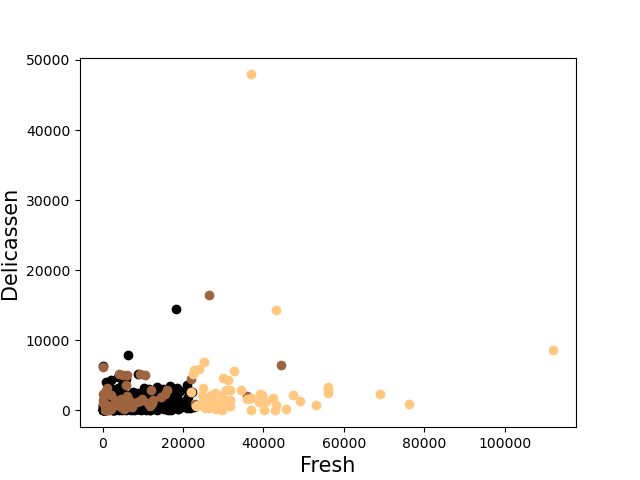
\includegraphics[width = \imWidth]{Fresh_Delicassen.png}} &
                \subfloat[Detergents\slash Paper vs Delicassen]{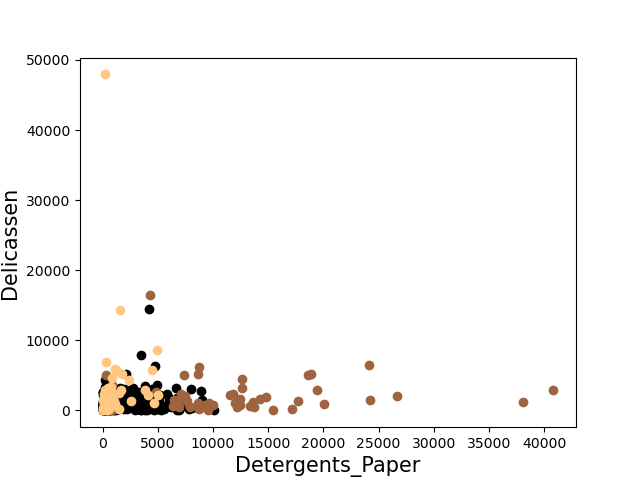
\includegraphics[width = \imWidth]{Detergents_Paper_Delicassen.png}}&
                \subfloat[Fresh vs Detergents\slash Paper]{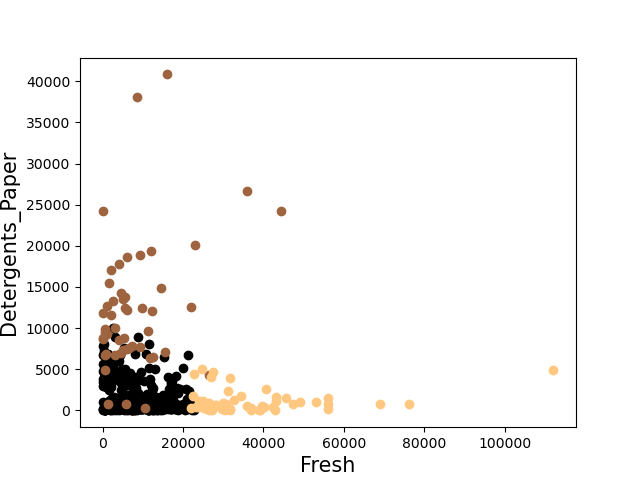
\includegraphics[width = \imWidth]{Fresh_Detergents_Paper.png}}\\
                \subfloat[Fresh vs Frozen]{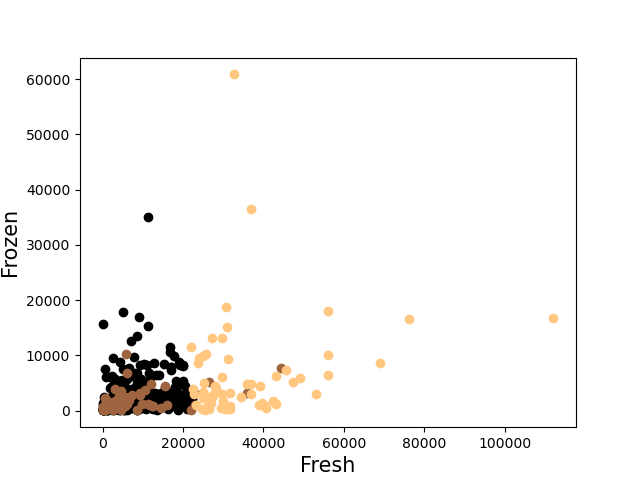
\includegraphics[width = \imWidth]{Fresh_Frozen.png}}&
                \subfloat[Fresh vs Grocery]{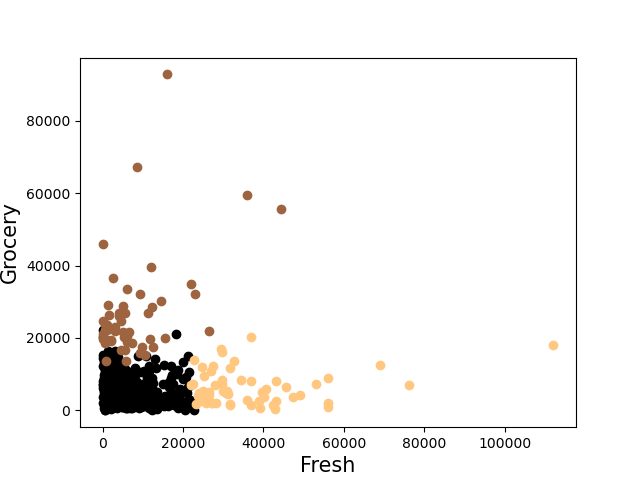
\includegraphics[width = \imWidth]{Fresh_Grocery.png}} &
                \subfloat[Fresh vs Milk]{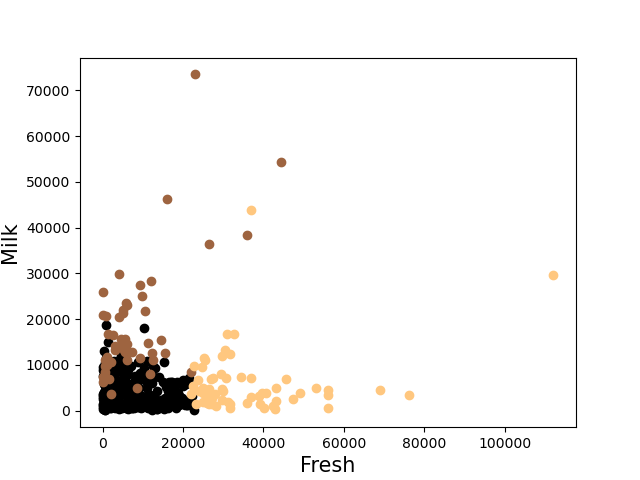
\includegraphics[width = \imWidth]{Fresh_Milk.png}}\\
                \subfloat[Frozen vs Delicatessen]{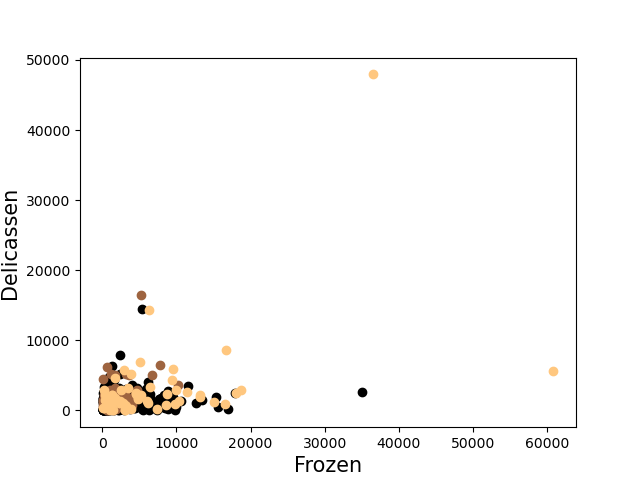
\includegraphics[width = \imWidth]{Frozen_Delicassen.png}} &
                \subfloat[Frozen vs Detergents\slash Paper]{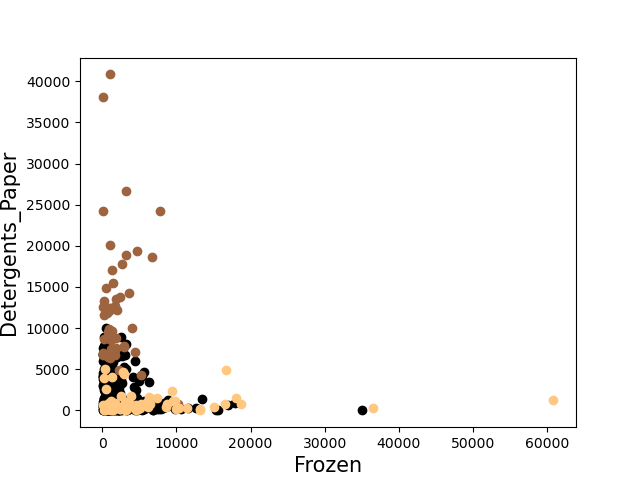
\includegraphics[width = \imWidth]{Frozen_Detergents_Paper.png}}&
                \subfloat[Grocery vs Delicatessen]{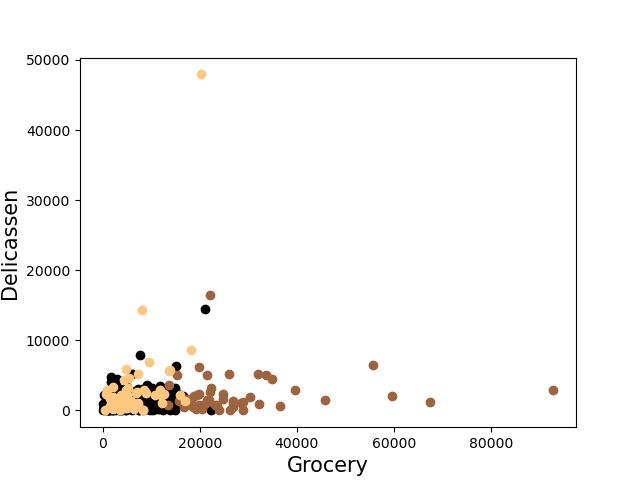
\includegraphics[width = \imWidth]{Grocery_Delicassen.png}}\\
                \subfloat[Grocery vs Detergents\slash Paper]{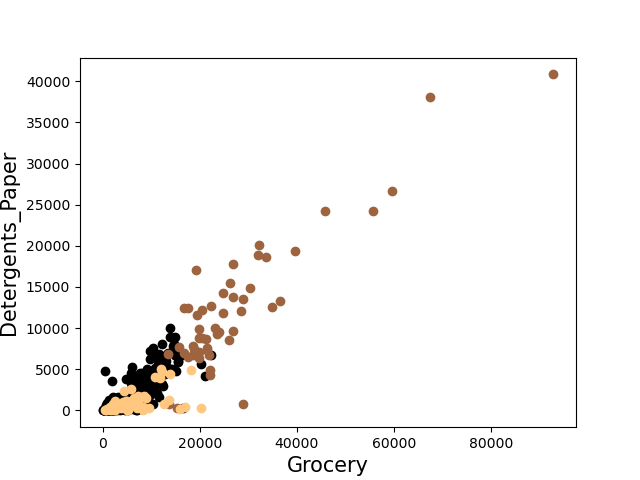
\includegraphics[width = \imWidth]{Grocery_Detergents_Paper.png}}&
                \subfloat[Grocery vs Frozen]{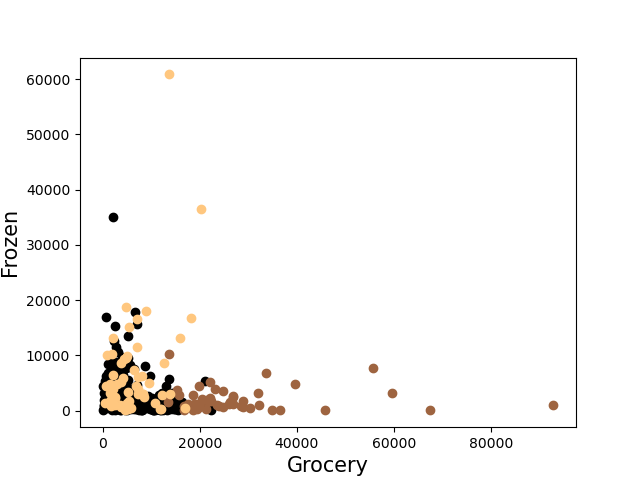
\includegraphics[width = \imWidth]{Grocery_Frozen.png}}&
                \subfloat[Milk vs Delicatessen]{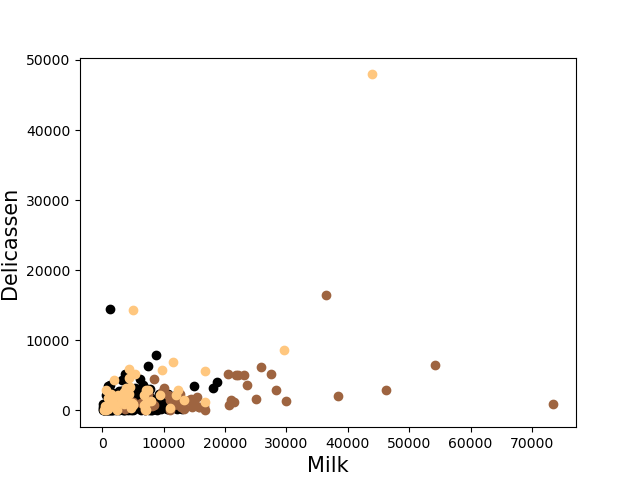
\includegraphics[width = \imWidth]{Milk_Delicassen.png}}\\
                \subfloat[Milk vs Detergents\slash Paper]{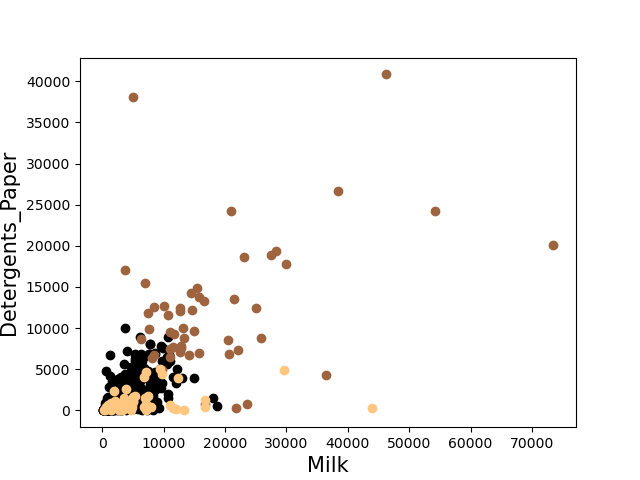
\includegraphics[width = \imWidth]{Milk_Detergents_Paper.png}}&
                \subfloat[Milk vs Frozen]{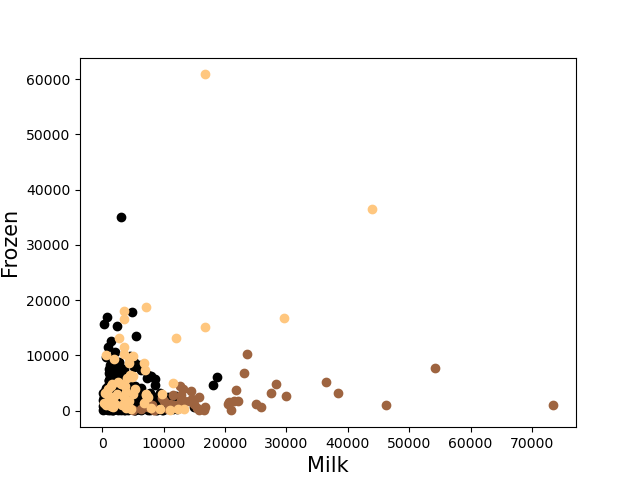
\includegraphics[width = \imWidth]{Milk_Frozen.png}}&
                \subfloat[Milk vs Grocery]{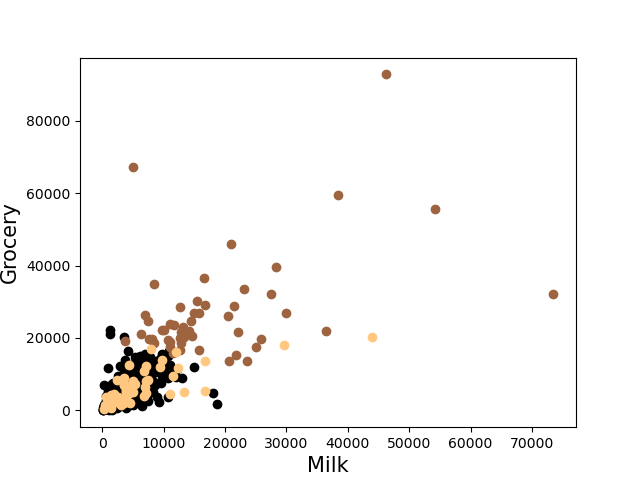
\includegraphics[width = \imWidth]{Milk_Grocery.png}}
                \end{tabular}
                \caption{Pairwise Scatterplots}
                \label{fig:figures} 
        \end{figure}









It should be noted that some pairwise attributes are better at separating the data than others, when using three clusters. In 
several of the scatterplots, the clusters overlap significantly, with little observable distinction between them. For example in
the `Frozen vs Delicatessen' plot, without the differentiation by the group colours, it would be impossible to tell by visual
observation which datapoints belonged to which cluster. If the dimensionality of the entire dataset were to be reduced for 
simplification, it would make sense to keep only one attribute in this pair. The same can be said for the majority of the pairs.
In fact, the only pairs with much visually observable distinction betweeen clusters are `Fresh vs Grocery', `Fresh vs Milk',
`Grocery vs Detergents/Paper', and still this observation is subjective. \\

There is a strong linear correlation between Grocery and Detergents/Paper, suggesting an increase in one of these attributes
would be observed with a rise in the other. A less strong, but still present, linear relationship exists with Milk and Grocery, 
and Milk and Detergents/Paper.\\ 

For many of the pairs containing Delicatessen, it appears there is inelastic expenditure on Delicatessen, where high expenditure in the
opponent attribute gives little to no rise in expenditure on Delicatessen. For example in the Grocery vs Delicatessen pair, the rise in
expenditure in Grocery yields little growth in expenditure on Delicatessen. Perhaps even stronger examples are the `Fresh vs Delicatessen',
and `Detergents/Paper vs Delicatessen pairs. There are some outliers present in the data, though this relationship with Delicatessen to 
other attributes may suggest Delicatessen expenditure is consistent, or not considered a choice, meaning the demand for Delicatessen is 
more inelastic, despite always being low.\\


\subsection{Cluster Evaluation} 

\noindent This section contains the cluster evaluation for different values of k in the K-means calculation. The three values of k evaluated
were the set \{3,5,10\}. As part of the cluster evaluation, the between-cluster score is calculated. This measures the separation of the clusters from one-another.
This will return a high value if the clusters are separated well.The within-cluster score was also calculated. This is a measure of the cluster density, which, for good clusters, should also be high.\\
To compare the clustering between these different k values, the ratio of between-cluster score to within-cluster score was calculated.\\
The results are shown in Table \ref{table:kvals}, rounded to 4 significant figures.
\vspace{4mm}

{\begin{table}
        \centering
        
\begin{tabular}{ c|c|c|c|}
        \cline{2-4} & \multicolumn{3}{|c|}{K-Value}\\
        \cline{2-4} & 3 & 5 & 10\\
        \hline
        \multicolumn{1}{|c|}{BC Scores} & 3132200000 &  25621000000 & 216500000000 \\
        \multicolumn{1}{|c|}{WC Scores} & 80330000000 &  52930000000 &  29650000000\\
        \multicolumn{1}{|c|}{BC/WC Ratio} & 0.03899 & 0.4841 &  7.301\\
        \hline
        \multicolumn{1}{|c|}{Calinksi-Harabaz's} & 210 &  215 & 206\\

        \hline

       \end{tabular}

        \caption{BC,WC and BC/WC Ratios}
        \label{table:kvals}

\end{table}}




\vspace{4mm}
The BC/WC ratio on its own is a relatively useless metric due to the different k values, so it must be normalised. To do this, the Calinski-Harabasz
index  was used. The Calinski-Harabasz index is a measure of separation and density of clusters. To score highly, the clusters should be well separated and
dense. This index showed the best k-value was 5, with a score of 215. Following this were 3 then 10, with scores of 210 and 206 respectively. The calculated values of this index are shown in Table \ref{table:kvals}.

Of the set, where k = 5 was the best performing K-means value at splitting the data, with respect to the C-H index. 

\vspace{4mm}


% {\begin{table}
%         \centering
% \begin{tabular}{ |c||c|c|c|}
%         \hline
%         Metric & 3 & 5 & 10\\
%         \hline
%         Calinksi-Harabaz's & 210.1 &  215.06 & 206.17\\
%         \hline
%        \end{tabular}

% \caption{Calinski-Harabasz Index}
%         \label{table:cali}
% \end{table}

\end{document}